\documentclass{article}
\usepackage{ctex}
\usepackage{geometry}
\usepackage{amsfonts,amssymb}
\usepackage{listings} 
\usepackage{fontspec}
\usepackage{graphicx}
\geometry{a4paper,left=2cm,right=2cm,top=1.5cm,bottom=1.5cm}
\renewcommand{\baselinestretch}{1.1}
\title{科学计算作业2}	
\author{张文涛 517030910425}
\date{\today}
\lstset{columns=flexible,numbers=left,numberstyle=\tiny,basicstyle=\small,keywordstyle=\color{blue!70},commentstyle=\color{red!50!green!50!blue!50}, rulesepcolor= \color{ red!20!green!20!blue!20} }
\begin{document}
	\maketitle
	\begin{itemize}
		\item[1.]给定离散点$x_{i}, i = 0,1,\cdots,n+1$,及$y_{i}, i = 40,1,\cdots,n+1$,记$q(x)$为相应于点集$\{(x_{i},y_{i}):i=0,1,\cdots,n\}$的$n$次Langrange插值多项式,而$r(x)$为相应于点$\{(x_{i},y_{i}):i=1,2,\cdots,n+1\}$的$n$次Langrange插值多项式,定义\[p(x) = \frac{(x-x_{0})r(x) - (x-x_{n+1})q(x)}{x_{n+1}-x_{0}}\]
		试证明:$p(x)$为相应于点集$\{(x_{i},y_{i}):i=0,1,\cdots,n+1\}$的$n+1$次Lagrange插值多项式。\\\\
		证明:首先易得$r(x)$与$q(x)$为$n$次多项式,由此可推出$p(x)$为$n+1$次多项式。\\
		另对于式\[p(x) = \frac{(x-x_{0})r(x) - (x-x_{n+1})q(x)}{x_{n+1}-x_{0}}\]
		$\forall x_{i}, i = 1, 2, 3\cdots,n$,代入得到\[p(x_{i})=\frac{(x_{i} - x_{0})y_{i} - (x_{i} - x_{n+1})y_{i}}{x_{n+1} - x_{0}} = y_{i}\]
		对于$x_{n+1},x_{0}$,:
		\[p(x_{0})=\frac{-(x_{0}-x_{n+1})y_{0}}{x_{n+1}-x_{0}} = y_{0}\]
		\[p(x_{n+1})=\frac{(x_{n+1}-x_{0})y_{n+1}}{x_{n+1}-x_{0}} = y_{n+1}\]
		由此可证$p(x)$为相应于点集$\{(x_{i},y_{i}):i=0,1,\cdots,n+1\}$的$n+1$次插值多项式。\\
		再证$p(x)$为Lagrange插值多项式,设$l_{k_{p(x)}}(x)$为$p(x)$的插值基函数,$l_{k_{q(x)}}(x),l_{k_{r(x)}}(x)$为$q(x)$与$r(x)$的插值基函数\\
		由题意得:
		\[l_{k_{q(x)}}(x) =\frac{\prod_{i = 0, i \ne k}^{n}(x-x_{i})}{\prod_{i = 0, i \ne k}^{n}(x_{k}-x_{i})}\]
		\[l_{k_{r(x)}}(x) =\frac{\prod_{i = 1, i \ne k}^{n+1}(x-x_{i})}{\prod_{i = 1, i \ne k}^{n+1}(x_{k}-x_{i})}\]
		可以展开通分计算:
		\[\frac{(x-x_{0})l_{k_{r(x)}}(x)y_{k} - (x-x_{n+1})l_{k_{q(x)}}(x)y_{k}}{x_{n+1}-x_{0}}\]
		\[=\frac{\frac{\prod_{i=0, i\ne k}^{n+1}(x-x_{i})}{\prod_{i=0, i\ne k}^{n+1}(x_{k}-x_{i})}(x_{n+1} - x_{0})}{x_{n+1}-x_{0}}y_{k} = l_{k_{p(x)}}(x)y_{k}\]
		最后两边求和即得证。
		\\
		\item[2.]设$f(x)\in \mathbb{P}_{n}$,且对$k =  0,1,2\cdots,n$成立$f(k)=\frac{k}{k+1}$,试求多项式$f(x)$\\\\
		由题意可知$f(x)$为$n$次多项式,因为$f(k)=\frac{k}{k+1}$,所以可知方程$(x+1)f(x) = x$有$n$个根,分别为$x =  0,1,2\cdots,n$,由代数学基本定理,方程$(x+1)f(x)-x=0$可以表示为\[A\prod_{k=0}^{n}(x-k) = 0\]
		从而得到
		\[(x+1)f(x) = A\prod_{k=0}^{n}(x-k)+ x\]
		记$q(x) = A\prod_{k=0}^{n}(x-k)+ x$又已知$f(x)$为$n$次多项式,所以$q(x)$中必有因子$x+1$,即$q(-1) = 0$,将$-1$代入得:
		\[q(-1) = A(-1)^{n+1}(n+1)! - 1 = 0\]
		从而解得:
		\[A = \frac{1}{(-1)^{n+1}(n+1)!}\]
		所以:
		\[p(x) = \frac{\frac{\prod_{k=0}^{n}(x-k)}{(-1)^{n+1}(n+1)!} + x}{x+1}\]\\
		\item[3.]设$l_{0},l_{1}\cdots l_{n}$是以$x_{0},x_{1}\cdots x_{n}$为节点的$n$次Lagrange插值基函数,试证明:
		$$ \sum_{k=0}^{n}l_{k}(0)x_{k}^{j}=\left\{
		\begin{array}{rcl}
		0,       &      & {j = 1, 2 \cdots n}\\
		(-1)^{n}x_{0}x_{1}\cdots x_{n}     &      & {j = n+1}\\
		\end{array} \right. $$
		证明:考虑$f(x)=x^{j}$的Lagrange的插值余项,由Lagrange插值预想相关知识可得$f(x) = x^{j}$的$p(p \le j - 1)$次插值余项为:
		\[R_{n}(x) = x^{j} - L_{n}(x)=\frac{j!x^{j - p - 1}}{(n+1)!(j - p - 1)!}\prod_{i = 0}^{p}(x - x_{i})\]
		当$j = 1, 2\cdots n, p = n$时,$p > j - 1$,所以等式右边为$0$(因为多次求导使得$f(x) = x^{j}$变为$0$),考虑$L_{n}(x)$:
		\[L_{n}(x) = \sum_{k=0}^{n}l_{k}(x)x_{k}^{j} = x^{j}\]
		令$x = 0$,即得$\sum_{k=0}^{n}l_{k}(0)x_{k}^{j} = 0$\\
		当$j = n+1,p =n$时,代入得:
		\[x^{j} - \sum_{k=0}^{n}l_{k}(0)x_{k}^{j} = \frac{(n+1)!x^{0}}{(n+1)!1!}\prod_{i = 0}^{n}(x - x_{i})\]
		令$x = 0$,计算得到:
		\[\sum_{k=0}^{n}l_{k}(0)x_{k}^{j} = -(-1)^{n+1}x_{0}x_{1}\cdots x_{n}\]\\
		\item[4.]假设$n\ge 1,x_{j}$是区间$[-1,1]$上的等距节点,即$x_{j}=\frac{2j -n}{n},j = 0,1,\cdots n$,记$\omega_{n+1}(x) = (x - x_{0})\cdots (x - x_{n})$,试证明:\\
		(1)$\omega_{n+1}(1 - \frac{1}{n}) = \frac{(2n)!}{2^{n}n^{n+1}n!}$.\\
		(2)当$n$较大时,$\omega_{n+1}(1 - \frac{1}{n}) \sim -\frac{2^{n + \frac{1}{2}}e^{-n}}{n}$.\\\\
		由题:
		\[\omega_{n+1}(1 - \frac{1}{n}) = \prod_{i = 0}^{n}(x - x_{i})\]
		将$x = 1-\frac{1}{n},x_{i} =\frac{2i - n}{n}$代入得
		\[\omega_{n+1}(1 - \frac{1}{n}) = \prod_{i = 0}^{n}\frac{2(n-i) - 1}{n} = \frac{-(2n - 1)!!}{n^{n + 1}} = -\frac{(2n)!}{(2n)!!n^{n+1}} =-\frac{(2n)!}{n!2^{n}n^{n+1}}\]
		再利用Stirling公式,代入得
		\[\omega_{n+1}(1 - \frac{1}{n}) = -\frac{2\sqrt{\pi n}(\frac{2n}{e})^{2n}}{\sqrt{2 \pi n}(\frac{n}{e})^n 2^{n} n^{n+1}} = -\frac{2^{n + \frac{1}{2}}e^{-n}}{n}\]\\\\
		\item[5.]根据$f(x)=3^{x}$,取插值节点$-1,0,1$,利用MATLAB编程实现Lagrange插值,并计算$\sqrt[3]{3}$.\\\\
		编写程序如下:\\
			\begin{lstlisting}[language= MATLAB] 
				function ret=lagrange(x,y,xi)
				m=length(x);
				n=length(y);
				res = length(xi);
				if m ~= n , error('len(x)!=len(y)'); end;
				s=0;
				for i=1 : n
					z=ones(1,res);
					for j=1 : n
						if j ~= i
							z=z.*(xi-x(j))./(x(i)-x(j));
						end
					end
					s=s+z.*y(i);
				end
				ret=s;
			\end{lstlisting}
		将$x = [-1, 0, 1], y = 3.^x, t = 1/3$分别作为$x, y, xi$参数输入程序得到插值计算结果$\sqrt[3]{3} = 1.5185$\\
		\item[6.]设$f(x) = \frac{1}{1 + x^{2}},x \in [-5,5]$,在区间中给出等距节点,利用MATLAB分别作出$3$次Lagrange插值多项式,$6$次Lagrange插值多项式,$9$次Lagrange插值多项式,$10$次Lagrange插值多项式,并将它们与$f(x)$的图像比较。\\\\
		利用上题编写的插值函数,并再次编写作图程序,得到图象:\\
		\begin{lstlisting}[language = MATLAB]
			function ret = lagrangePic()
			xo = [-5:0.01:5];
			x3 = [-5:10/3:5];
			x6 = [-5:10/6:5];
			x9 = [-5:10/9:5];
			x10 = [-5:10/10:5];
			yo = 1./(1 + xo.^2);
			y3 = 1./(1 + x3.^2);
			y6 = 1./(1 + x6.^2);
			y9 = 1./(1 + x9.^2);
			y10 =1./(1 + x10.^2);
			plot(xo, yo, 'DisplayName', '原始图像');
			hold on;
			plot(xo, lagrange(x3, y3, xo), 'DisplayName', '三次插值');
			plot(xo, lagrange(x6, y6, xo), 'DisplayName', '六次插值');
			plot(xo, lagrange(x9, y9, xo), 'DisplayName', '九次插值');
			plot(xo, lagrange(x10, y10, xo), 'DisplayName', '十次插值');
			hold off;
		\end{lstlisting}
		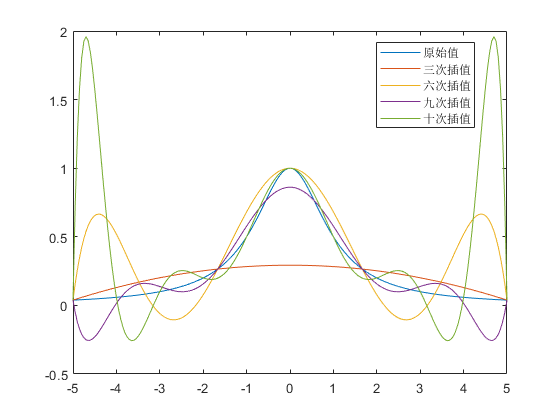
\includegraphics[scale=1]{Lagrange.png}\\\\
		可以观察到在插值次数增加后图象中间部分近似得较好,而两边偏差较大。
	\end{itemize}
\end{document}